\documentclass[AutoFakeBold,a4paper]{ctexart}
\usepackage{graphicx}
\usepackage{titlesec}
\usepackage{ctex}
\usepackage{xeCJK}
\usepackage{fontspec}
\usepackage{amsmath}
\usepackage{array}
\usepackage{listings}
\usepackage{color, xcolor}
\usepackage{caption}
\usepackage{float}
\usepackage{amsthm,txfonts}
\usepackage{amssymb}
%\usepackage{euler}
\usepackage{fancyhdr}
\usepackage[colorlinks,linkcolor=magenta,citecolor=magenta]{hyperref}
\usepackage{multicol}
\usepackage{titletoc}
\usepackage[biblabel]{cite}
\usepackage[left=1.25in,right=1.25in,top=1in,bottom=1in]{geometry}

\renewcommand\lstlistingname{代码}
%\setCJKmainfont{微软雅黑}[BoldFont=SimHei, ItalicFont=KaiTi]

\pagestyle{fancy}

\fancyhead[RO, RE]{\thepage}
\fancyhead[LO, LE]{\kaishu \leftmark}
\fancyhead[CO, CE]{}

\fancyfoot[RO, RE]{}%lhy1210302421@mail.ustc.edu.cn}
\fancyfoot[LO, LE]{{\kaishu \today}}
\fancyfoot[CO, CE]{}

\setmainfont[Ligatures=TeX]{CMU Serif}
\setsansfont[Ligatures=TeX]{CMU Sans Serif}
\setmonofont[Mapping=]{CMU Typewriter Text}

\setCJKmainfont{PingFangSC-Regular}[BoldFont=PingFangSC-Medium]

\renewcommand{\headrulewidth}{0.1mm} 
\renewcommand{\footrulewidth}{0.1mm}

\lstset{
    basicstyle          =   \sffamily,          % 基本代码风格
    keywordstyle        =   \bfseries,          % 关键字风格
    commentstyle        =   \rmfamily\itshape,  % 注释的风格,斜体
    stringstyle         =   \ttfamily,  % 字符串风格
    flexiblecolumns,                % 别问为什么,加上这个
    numbers             =   left,   % 行号的位置在左边
    showspaces          =   false,  % 是否显示空格,显示了有点乱,所以不现实了
    numberstyle         =   \zihao{-5}\ttfamily,    % 行号的样式,小五号,tt等宽字体
    showstringspaces    =   false,
    captionpos          =   t,      % 这段代码的名字所呈现的位置,t指的是top上面
    frame               =   lrtb,   % 显示边框
    captionpos          =   b       % caption的位置(填t在上,填b在底部)
}

\lstdefinestyle{Python}{
    language        =   Python, % 语言选Python
    basicstyle      =   \zihao{-5}\ttfamily,
    numberstyle     =   \zihao{-5}\ttfamily,
    keywordstyle    =   \color{blue},
    keywordstyle    =   [2] \color{teal},
    stringstyle     =   \color{magenta},
    commentstyle    =   \color[rgb]{0.416,0.6,0.3333}\ttfamily,
    breaklines      =   true,   % 自动换行,建议不要写太长的行
    columns         =   fixed,  % 如果不加这一句,字间距就不固定,很丑,必须加
    basewidth       =   0.5em,
}

\lstdefinestyle{C}{
    language        =   C, % 语言选Python
    basicstyle      =   \zihao{-5}\ttfamily,
    numberstyle     =   \zihao{-5}\ttfamily,
    keywordstyle    =   \color{blue},
    keywordstyle    =   [2] \color{teal},
    stringstyle     =   \color{magenta},
    commentstyle    =   \color[rgb]{0.416,0.6,0.3333}\ttfamily,
    breaklines      =   true,   % 自动换行,建议不要写太长的行
    columns         =   fixed,  % 如果不加这一句,字间距就不固定,很丑,必须加
    basewidth       =   0.5em,
}

% \providecommand{\keywords}[1]{\textbf{\textit{关键字:}} #1}

% \renewcommand{\abstractname}{\textbf{摘要:}}

\begin{document}

\title{\textbf{\Huge 大作业-可行性报告}}

\author{陈思睿 \quad 梁恒宇 \quad 吕泓涛 \quad 汤力宇\\
中国科学技术大学 \quad 安徽合肥}

\date{\today}

\maketitle

\ctexset { section = { format={\Large \bfseries} } }
\ctexset { subsection = { format={\large \bfseries} } }

\titlecontents{section}[2em]{\addvspace{1.3mm}\bf}{%
\contentslabel{2.0em}}{}{\titlerule*[5pt]{$\cdot$}\contentspage}

\titlecontents{subsection}[4.2em]{}{\contentslabel{2.5em}}{}{%
\titlerule*[5pt]{$\cdot$}\contentspage}

\titlecontents{subsubsection}[7.2em]{}{\contentslabel{3.3em}}{}{%
\titlerule*[5pt]{$\cdot$}\contentspage}

\pagenumbering{roman}
\tableofcontents

\pagenumbering{arabic}
\setcounter{page}{1}

% \section{小组成员}

% \begin{itemize}
%     \item 陈思睿
%     \item 梁恒宇
%     \item 吕泓涛
%     \item 汤力宇
% \end{itemize}

\section{项目介绍}

\textbf{使用新兴的eBPF架构,实现兼有安全性和性能的通用沙箱。}

任何操作系统都或多或少的潜藏着安全漏洞,
近年来各大主流OS都被爆出过存在重大安全隐患。
当恶意程序侵入用户的系统,则可能破坏、窃取宝贵的用户数据,
造成不可估量的损失。而为了防止此类事件发生,沙盒技术正在不断发展。
沙盒技术通过对可疑的进程进行隔离与监控,
防止其对系统其它部分造成损害。

然而随着恶意程序的攻击策略不断扩展,
传统沙盒的安全性也难以长期保持,因此一个理想的沙盒应当在高效、
安全同时拥有便于升级维护的特点,这一理想在现有的沙盒中难以实现。
用户态的沙盒存在着大量到内核态的状态切换,带来了严重的性能损失,
而内核态的沙盒则在损失了升级的灵活性的同时带来了更多可能被攻击的安全漏洞。

面对这一困境,本项目希望使用新兴的eBPF架构,
实现一个可以从用户态灵活对其升级的内核态沙盒。
由于BPF架构的设计特征,这一沙盒将不会给内核多带来额外的安全漏洞,
并且将可以实现和内核态相仿的性能。

\section{理论依据}

% 结构、安全、性能分析

\section{技术依据}

\subsection{BPF应用实现}

\subsubsection{一个简单的BPF程序}

运行BPF程序需要两个部分,一个是BPF内核程序,一个是用户态的加载程序。
BPF内核程序需要编译成BPF内核字节码,用户态程序只需要编译成可执行文件。

加载进内核的程序可以使用C代码编写,示例C代码如下:

\lstinputlisting[style=C,caption=BPF内核程序代码]{../LiangHengyu/hello_world/bpf_program.c}

程序被设置为在其他程序开始执行时被调用,并输出“Hello World!”。

它将被编译成字节码:

\lstinputlisting[style=C,caption=BPF字节码]{../LiangHengyu/hello_world/bpf_program_asm.txt}

用户态程序如下,它基本上只起一个加载BPF程序的作用:

\lstinputlisting[style=C,caption=BPF加载程序]{../LiangHengyu/hello_world/loader.c}

执行BPF程序,需要以管理员身份调用该加载程序。程序的执行效果如下图所示:

\begin{figure}[H]
    \centering
    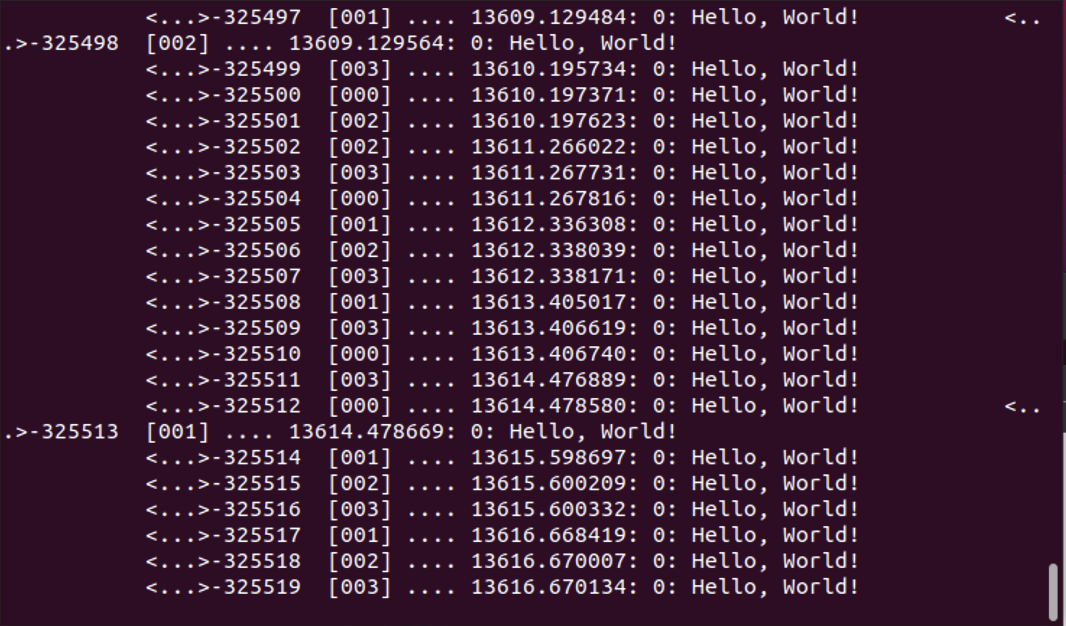
\includegraphics[width=0.7\columnwidth]{../LiangHengyu/hello_world/test1.png}
    \caption{示例程序执行效果}
\end{figure}

\subsubsection{seccomp实现控制系统调用}

这个程序会拒绝被调用程序的所有和写相关的系统调用。

\subsection{Linux内核BPF源码修改}

\section{技术路线}

\begin{enumerate}
    \item 在seccomp结构上优化制作更好的系统调用的拦截和判断机制,
    实现只通过一个简单的过滤器就能保证较强安全性的轻量级安全沙盒。
    \item 尝试将一个基于虚拟化技术的安全沙盒通过bpf程序的方式制作出来并且诸如OS内运行,
    可能需要修改现有的ebpf认证与导入机制。
    \item 仅将bpf程序作为劫持和修改系统调用的小模块,
    将其结合到某个现有的用户态沙盒中,从而优化某个用户态沙盒应用的效率。
\end{enumerate}

\bibliography{../paper.bib}
\bibliographystyle{ieeetr}

\end{document}